\documentclass[10pt]{article}
\usepackage[pdftex]{graphicx}
\usepackage{amssymb, amsmath}
\usepackage{url}

\usepackage{fullpage}
\setlength{\parindent}{0pt}
\setlength{\parskip}{\baselineskip}

\title{Implementation of the Density Evolution method with
Fokker-Plank for L-NLIF Model in Python}
\author{Valentin Haenel \\
valentin.haenel@gmx.de \\
BCCN Berlin}

\begin{document} 

\maketitle

\section{Introduction}

This report is a description of the work done by Valentin Haenel
for a Lab Rotation within the Bernstein Center for Computational
Neuroscience in Berlin. The rotation was completed in the lab of Gabriel
Curio under the supervision of Bartosz Telenczuck. 

Throughout the project I have implemented a variant of the Leaky
Integrate and Fire Neuron(LIF), and a method to fit the parameters of this
neuron using a model of the input and extracellularly recorded spikes.
Primarily this involved solving a partial differential equation and constructing
a maximum likelihood objective function. 


\section{Model}
The original model is a L-NLIF model, which consists of a Linear
(L) Filter, followed by a probabilistic or Noisy (N) form of Leaky
Integrate and Fire spike generation(LIF) (Paninski et
al.\cite{PaninskiPillowSimoncelli}). For sake of completeness the
model is briefly described here.

The evolution of the Voltage $V$ is given by:
\begin{equation}
    dV = (-g(V(t) -V_{leak}) +I_{stim}(t) + I_{hist}(t)) dt + W_{t}
\end{equation}
Where $g$ is the leak conductance $V_{leak}$ is the leak reversal
potential $I_{stim}$ is the convolution of linear filter with the
input signal, $I_{hist}$ is the spike current history and $W_t$ is
standard Gaussian white noise. More precisely:
\begin{equation}
    I_{stim}(t) = \vec{k} \cdot  \vec{x}(t) 
\end{equation}
\begin{equation}
    I_{hist}(t) = \sum_{j=0}^{i-1}h(t-t_j)
\end{equation}
Where $k$ is a linear filter and $h$ is a fixed postspike current waveform. 

\section{Algorithms}

This section describes the algorithms employed.

\subsection{PDE Solver}

\subsubsection{The Problem}
Let 
\begin{equation}
    P(V,t) \equiv P(V(t) \cap  V(s) < V_{th} \forall s < t)
\end{equation}
This refers to the probability of $V(t)$, the membrane potential,
being less than $V_{th}$ the firing threshold until time $t$.  

As stated in \cite{PaninskiPillowSimoncelli} the method of density
evolution requires us to solve the
following Fokker-Planck drift diffusion equation numerically.
\begin{equation}
    \frac{\partial P(V,t)}{\partial t} =
    \frac{\sigma^2}{2} \frac{\partial^2 P(V,t) } {\partial V^2} +
    g\frac{\partial[(V-V_{rest})P(V,t)]}{\partial V}
    \label{fokkerplanck}
\end{equation}

We will be solving the evolution of the probability density for a
given inter spike interval(ISI). And therefor we will constrain the range
of $V$ and $t$.
\begin{equation}
    P(V_{th},t) = 0
    \label{boundarytop}
\end{equation}
\begin{equation}
    P(V,0) = \delta(V-V_{reset})
    \label{boundaryleft}
\end{equation}

Condition (\ref{boundarytop}) ensures that the probability of obtaining a spike
during an ISI is zero. Condition (\ref{boundaryleft}) ensures
that at the beginning of an ISI, i.e. at the time of the last spike,
the probability of the neuron being at reset potential is exactly one.
Thereby we have obtained the constraints for the top and the left had
side of our solution grid, however, when solving numerically we also
need a lower bound on the voltage $V_{lb}$, so this becomes an
additional boundary condition, for the  bottom:
\begin{equation}
    P(V_{lb},t) = 0 
    \label{boundarybottom}
\end{equation}

Ideally $V_{lb} = -\infty $.

$V_{rest}$ is defined as the stationary point of the noiseless
subthreshold dynamics:
\begin{equation}
    V_{rest}(t) = V_{leak} + \frac{1}{g}(\vec{k} \cdot \vec{x}(t)
    \sum_{j=0}^{i-1}h(t-t_j))
\end{equation}


We can rewrite (\ref{fokkerplanck}) as:
\begin{equation}
    \frac{\sigma^2}{2} \frac{\partial^2 P(V,t) } {\partial V^2} +
    g(V-V_{rest})\frac{\partial P(V,t)}{\partial V} +
    gP(V,t) -
    \frac{\partial P(V,t)}{\partial t} = 
    0
\end{equation}
Since we know that:
\begin{equation}
    \frac{\partial[(V-V_{rest})P(V,t)]}{\partial V} =
    \frac{\partial (V-V_{rest})}{\partial V}  P +
    \frac{\partial P}{\partial V} (V-V_{rest})
\end{equation}
and
\begin{equation}
    \frac{\partial (V-V_{rest})}{\partial V} = 1
\end{equation}

\subsubsection{Finite Differencing}

In order to solve (\ref{fokkerplanck}) numerically we discretize time
and potential. We adopt the notation that Potential is discretized
into $W$ intervals of length $w$ and indexed
by $\nu= 0,1, \dots W $.  Time is discretized  into $U$ intervals of
length $u$ and indexed by: $\tau= 0,1, \dots U $.
We adopt the notation: $P_{\nu,\tau} = P(\nu w,\tau u)$

A forward finite differencing scheme would like:
\begin{eqnarray}
    \hat{P} =& P_{\nu,\tau} \\
%
    \frac{\partial \hat{P}}{\partial t} =& \frac{P_{\nu,\tau +1 } -
    P_{\nu,\tau}}{u} \\
%
    \frac{\partial \hat{P}}{\partial V} =& 
    \frac{P_{\nu +1,\tau } -
    P_{\nu - 1,\tau } }
    {2w} \\
%
    \frac{\partial^2 \hat{P}}{\partial V^2} =& 
    \frac{P_{\nu+1,\tau} - 2 P_{\nu,\tau} + P_{\nu-1,\tau}}
    {w^2} 
\end{eqnarray}

However as suggested in \cite{PaninskiHaithSzirtes} we will use the
computationally more stable Crank-Nicolson scheme\cite{press}.  
We rewrite the derivatives using the new scheme which is centered around $t +
u/2$.

\begin{eqnarray}
    P_{CN} =& \frac{P_{\nu,\tau} + P_{\nu,\tau + 1}}{2} \\
    %
    \frac{\partial P_{CN}}{\partial t} =& \frac{P_{\nu,\tau +1 } -
    P_{\nu,\tau}}{u} \\
    %
    \frac{\partial P_{CN}}{\partial V} =&
    \frac{P_{\nu +1,\tau } + P_{\nu +1,\tau +1 } -
    P_{\nu - 1,\tau } - P_{\nu -1,\tau +1}} 
    {4w} \\
    %
    \frac{\partial^2 P_{CN}}{\partial V^2} =&
    \frac{P_{\nu+1,\tau} - 2 P_{\nu,\tau} + P_{\nu-1,\tau} +
    P_{\nu+1,\tau+1} - 2 P_{\nu,\tau+1} + P_{\nu-1,\tau+1}}
    {2w^2} 
\end{eqnarray}

\subsubsection{Tridiagonal Equations}

If we now let:
\begin{align*}
a &= \frac{\sigma^2}{2} \\
b &= g(V - V_{rest}) \\
c &= g \\
\end{align*}
and multiply throughout with $4w^2u$
we may rearrange all the $P_{*,\tau+1} $ terms on the left hand side:
\begin{multline}
    \overbrace{-(2au+bwu)}^{A_\nu} P_{\nu+1,\tau+1} + 
    \overbrace{(4au - 2cw^2u + 4w^2)}^{B_\nu} P_{\nu,\tau+1}
    \overbrace{-(2au-bwu)}^{C_\nu} P_{\nu-1,\tau+1}
    =  \\
    \underbrace{(2au+bwu) P_{\nu+1,\tau} +  
    (-4au +2cw^2u + 4w^2) P_{\nu,\tau} + 
    (2au-bwu) P_{\nu-1,\tau}}_{D_{\nu}}
    \label{rearrange}
\end{multline}
For each $ \nu = 1 , \dots , W-1 $

Using (\ref{rearrange}) we have obtained $W-1$ simultaneous equations which
we may now rewrite in the following tridiagonal matrix notation.
\begin{equation}
\underbrace{
\begin{pmatrix}
    B_0    & A_0   & 0      & 0      & \cdots  & 0       \\
    C_1    & B_1   & A_1    & 0      & \cdots  & 0       \\
    0      & C_2   & B_2    & A_2    & 0      &         \\
    \vdots &       & \ddots & \ddots & \ddots & \vdots  \\
    0      & \cdots & 0      & C_{W-1}& B_{W-1}& A_{W-1} \\
    0      & \cdots &        & 0      & C_W    & B_W     \\
\end{pmatrix}}_{\Lambda}
\underbrace{
\begin{pmatrix}
    P_{0,\tau+1}   \\
    P_{1,\tau+1}   \\
    P_{2,\tau+1}   \\
    \vdots         \\
    P_{W-1,\tau+1} \\
    P_{W,\tau+1}   \\
\end{pmatrix}}_{\chi}
=
\underbrace{
\begin{pmatrix}
    D_0     \\
    D_1     \\
    D_2     \\
    \vdots  \\
    D_{W-1} \\
    D_W     \\
\end{pmatrix}}_{\beta}
\end{equation}

However this matrix equation has W+1 equations, so we must use the
boundary conditions (\ref{boundarytop}) and
(\ref{boundarybottom}) to specify the first and last rows of $\Lambda$.
We can then use a tridiagonal matrix algorithm to solve $\Lambda \chi
= \beta$. This allows us to iteratively obtain the density evolution $P(V,t)$ of the
membrane potential for a given ISI. Where the initial $\beta$ for an ISI is given by
(\ref{boundaryleft}) and the halting criterion is the time of the next
spike. So for the $i$th spike we obtain values for $V$ in the range
$[V_{lb}, V_{th}]$ and for $t$ in the range $[t_{i-1},t_{i}]$. An
example can be seen in figure \ref{P_vt}.


\subsection{First Passage Time}

The maximum likelihood optimizer proposed in
\cite{PaninskiPillowSimoncelli} however uses the first passage time
density at a given time point which is defined as:

\begin{equation}
    fpt(t) = -\frac{\partial}{\partial t} \int P(V,t)dV
\end{equation}

and this can be easily computed from an $P(V,t)$ matrix by summing
across $P$ and finding differences across $t$.

\subsection{Maximum Likelihood Estimator}

Putting together the PDE Solver and method for computing the First
Passage Time 
The final likelihood is then simply

\begin{equation}
    L_{\vec{x},t_{i}} = \Pi_{i} fpt(t_{i})
\end{equation}

This is the product of the first passage time at the times of
spiking for all spikes.

The pseudocode for the objective function can be described as follows:

{\tt
for each spike interval do:
\begin{enumerate}
    \item compute $P(V,t)$ as matrix
    \item compute $fpt$ as vector
\end{enumerate}
return the product of the last scalars in the $fpt$ vectors.}

This objective function could be presented to a standard numerical
optimizer, for example the Nelder-Mead Downhill simplex \cite{press},
this needs no gradients and is fairly robust but slow.

\subsection{Monte Carlo Method}

To double check the results of the PDE Solver and the resulting First
Passage Time , we additionally implemented some basic monte carlo
simulations. This did not involve much more than simulating a few
thousand single spike runs of our model, with noise. The resulting
potential traces, and spike times were used to obtain both $P(V,t)$
and $fpt$. The density evolution is compared qualitatively and the
$fpt$ is compared using a Kolmogorov-Smirnov (K-S) test\cite{press}.


\section{Implementation}

This section describes the concrete implemenation

\subsection{Availability and Design}

The algorithm has been implemented in Python, and the full source code
has been made available within a revision control system under a free
software license at: http://github.com/esc/molif/tree/master. Given
that the Python Language was named after the British Comedians Monty
Python we decided to call the software {\it Meaning Of LIF},
(abbreviated to {\it molif}) which is a reference to the Monty Python
movie {\it Meaning of Life}. 

The software is structured into a series of modules contained within
the package {\tt molif} 

\begin{itemize}
    \item {\tt model} implementation of the neuron model
    \item {\tt density} implementation of the pde solver 
    \item {\tt likelihood} connects the optimizer and the pde solver
    \item {\tt montecarlo} implementation of monte carlo simulator
    \item {\tt plotting} methods used to generate plots
    \item {\tt util} methods to determine timing
\end{itemize}

The software uses the additional packages numpy, scipy for vector
based and scientific computing, and pylab/matplotlib for plotting the
results. We used the modules {\it scipy.sparse} and {\it
scipy.linsolve} for computing the solution to tridiagonal equations, and the
method {\it optimize.fmin}, which implements the Nelder-Mead Downhill
Simplex, for minimizing the negative likelihood.


\subsection{Limitations and Future Work}

The PDE solver uses sparse matrix algorithms to store and solve the
tridiagonal matrix. Ideally we would like to use the routine $TRIDAG$
described in \cite{press}, however an open source implementation in
python was not available, although feasible. This improvement could
possibly speed up the computation of $P(V,t)$.

There is a serious bug, whereby the value of sigma,
must be within a specific range of $0.1 - 0.05$, otherwise strange
oscillatory instabilities occur. Among the possible causes, are a
numerical instability in the finite differencing scheme, a bug in our
code, a bug in the solver for the linear equations or the
discretization of $V$ and $t$ being to large. 

Currently the gradient of the objective function isn't implemented,
and any gradient based optimizer would need to compute their
approximation from the function values. 

We used a Kolmogorov-Smirnov (K-S) test to check that the first
passage time computed by the pde-solver and the monte carlo method
come from the same distribution. However the test currently returns a
negative result, although at first glance the distributions look very
similar. 

Lastly we should mention that the objective function isn't fully
operational yet. A simple test is executed as follows: first we
generate some spikes with given parameters, and then we attempt to fit
parameters to these spikes. If the code operates correctly the
optimizer should not deviate away from the initial paramters vector.
However currently this is not the case and the optimizer finds a
minimum at a different position in parameter space.

\subsection{Images}

This section presents some plots.

Figure \ref{P_vt} shows the comparison of PDE Solver and Monte Carlo
method when computing the density evolution. The slight difference in angle may,
unfortunately, be a bug in the code.

Figure \ref{fpt} shows the comparison of the PDE Solver and Monte
Carlo method when computing the first passage time. Unfortunately a
K-S test allows us to reject the hypothesis that these two come from
the same distribution, even though they look very much alike at a
first glance.

\begin{figure}[htp]
\centering
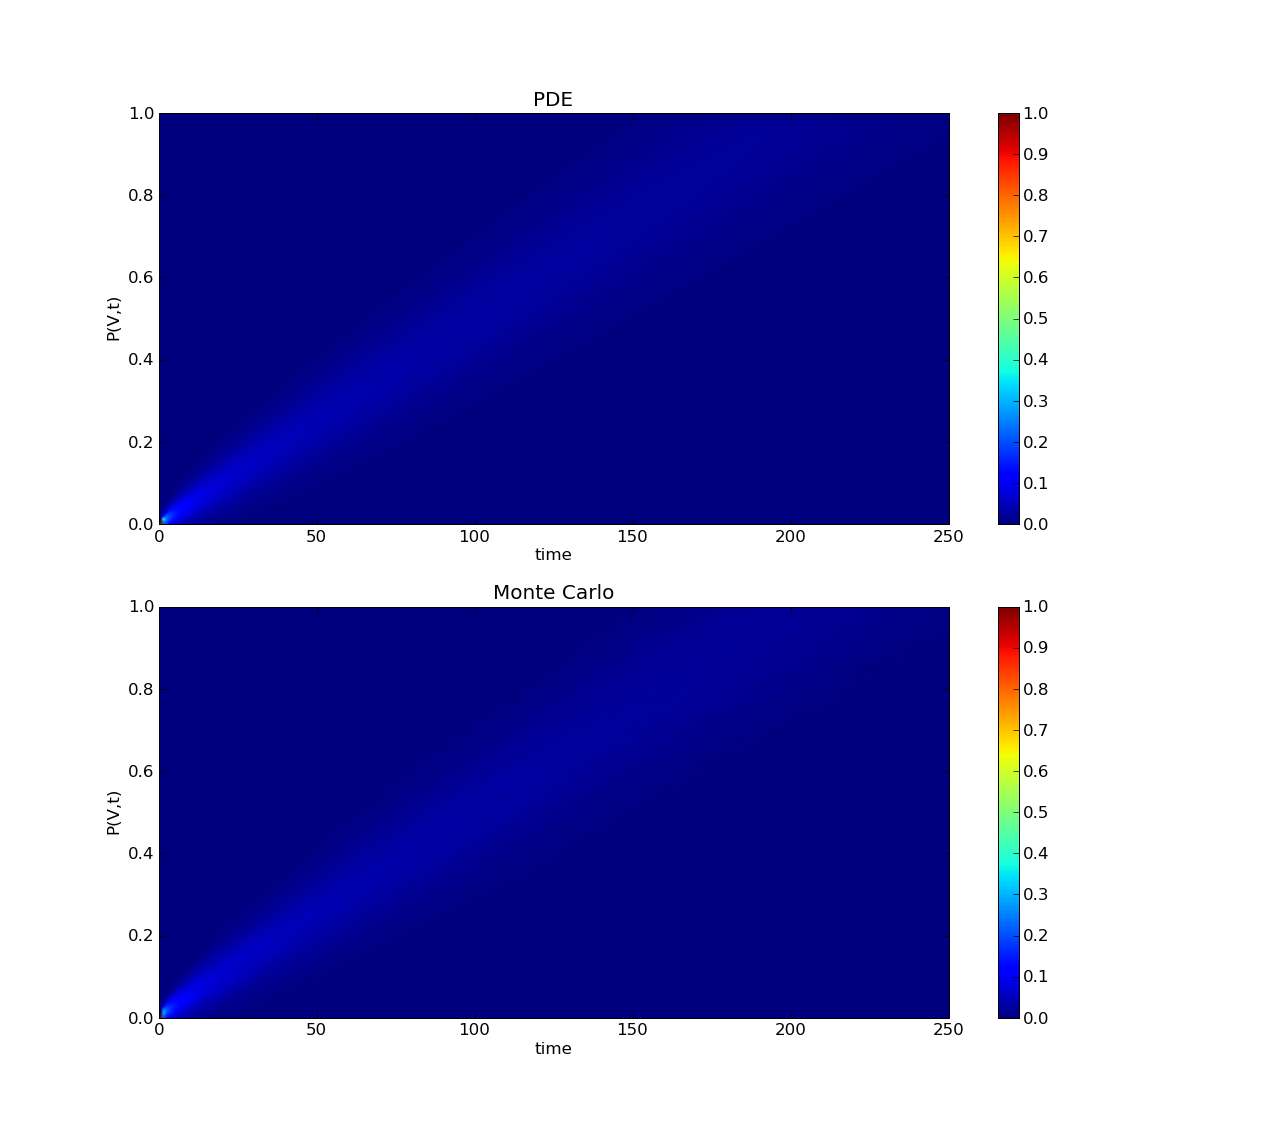
\includegraphics[scale=0.60]{P_vt}
\caption{Density Evolution}
\label{P_vt}
\end{figure}

\begin{figure}[htp]
\centering
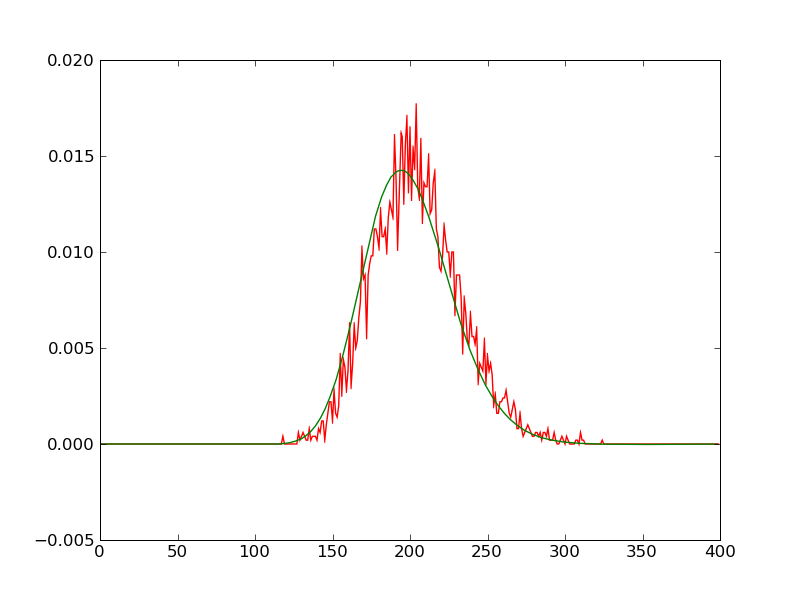
\includegraphics[scale=0.60]{fpt.png}
\caption{First Passage Time Comparison}
\label{fpt}
\end{figure}

\subsection{Conclusion}

Not all of the initial Porject Goals were reached to my full
satisfaction. We did implement an Integrate and Fire
neuron, and a method to fit the parameters, however we did not get as
far as actually fitting real experimental data. None the less 
useful code has been produced and solid numerical techniques (Solving
Partial Differential Equations) were
learnt, and I consider the lab rotation to be successful. 

\bibliography{documentation}{ \bibliographystyle{abbrv} }

\end{document}
